\documentclass[a4paper]{article}
\usepackage[utf8]{inputenc}
\usepackage{multicol}
\usepackage{paracol}
\usepackage{geometry}
\usepackage{amssymb}
\usepackage{graphicx}
\usepackage{wrapfig}
\usepackage{caption}
\usepackage{subcaption}
\usepackage{fancyhdr}
\usepackage[parfill]{parskip}
\usepackage{hyperref}
\usepackage{amsmath}
\usepackage{listings}
\usepackage[table]{xcolor}
\usepackage{mathtools}
\usepackage{array}
\usepackage{enumitem}
\usepackage{wrapfig}
\usepackage{svg}
\usepackage{algorithm2e}
\usepackage[edges]{forest}

% VS2017 C++ color scheme
\definecolor{clr-background}{RGB}{255,255,255}
\definecolor{clr-text}{RGB}{0,0,0}
\definecolor{clr-string}{RGB}{163,21,21}
\definecolor{clr-namespace}{RGB}{0,0,0}
\definecolor{clr-preprocessor}{RGB}{128,128,128}
\definecolor{clr-keyword}{RGB}{0,0,255}
\definecolor{clr-type}{RGB}{43,145,175}
\definecolor{clr-variable}{RGB}{0,0,0}
\definecolor{clr-constant}{RGB}{111,0,138}
\definecolor{clr-comment}{RGB}{0,128,0}

\lstset{
    language=Java,
    basicstyle=\ttfamily,
    keywordstyle=\color{blue}\ttfamily,
    stringstyle=\color{red}\ttfamily,
    commentstyle=\color{green}\ttfamily,
    morecomment=[l][\color{magenta}]{\#},
}

\lstset{
    language=Java,
    backgroundcolor=\color{clr-background},
    basicstyle=\color{clr-text}, % any text
    stringstyle=\color{clr-string},
    identifierstyle=\color{clr-variable}, % just about anything that isn't a directive, comment, string or known type
    commentstyle=\color{clr-comment},
    %directivestyle=\color{clr-preprocessor}, % preprocessor commands
    % listings doesn't differentiate between types and keywords (e.g. int vs return)
    % use the user types color
    keywordstyle=\color{clr-type},
    keywordstyle={[2]\color{clr-constant}}, % you'll need to define these or use a custom language
    tabsize=1,
    frame=single
}

\DeclareMathOperator*{\argmax}{arg\,max}
\DeclareMathOperator*{\argmin}{arg\,min}

\hypersetup{
    colorlinks,
    citecolor=black,
    filecolor=black,
    linkcolor=black,
    urlcolor=black
}

\geometry{
 a4paper,
 left=18mm,
 right=18mm,
 top=25mm,
 bottom=25mm
}

\graphicspath{{./images/}}
\pagestyle{fancy}

% custom
\usepackage{float}
\usepackage[skip=0pt]{caption}
\setlength{\intextsep}{5pt plus 1pt minus 1pt}

\title{\vspace{-20mm}A Quorum-Based Total Order Broadcast Protocol for Distributed Intelligence Databases}
\author{Dalla Croce Enrico, Dematté Luca}
\date{Distributed Systems 1 Project -- \today}

\begin{document}
    \maketitle
    \section{Project Structure}
        \subsection{Subpackage}
            We created a subpackage named \lstinline|cs| located at \lstinline|it.unitn.ds.cs|.
            The code related to our abstractions is located under the \lstinline|cs| package.
        \subsection{Naming Convention}
            To easily identify our classes all class names have the prefix \lstinline|CS|.
    \section{Design}
        To keep the explanation concise, we focus solely on the aspects that complement the project instructions:\\
        our assumptions, additional features, and custom solutions.
        \subsection{Assumptions}
            \subsubsection{Project Instructions}
                \begin{itemize}
                    \item Communication channels are assumed to be reliable and FIFO
                    \item A strict majority of replicas never crashes.
                    \item Replicas fail by crashing and do not recover.
                    \item Static system membership: no new replicas may join after initialization.
                \end{itemize}
            \subsubsection{UUID uniqueness}
                We assume that the generated UUIDs are unique. Replicas independently generate UUIDs and so technically it can happen that two independent UUIDs match, making them not unique.\\
                It has to be noted that we rely on the UUID class included in the Java SDK which offers some guarantees.\\
                The documentation for the method \lstinline|public static UUID randomUUID()| states: "The UUID is generated using a cryptographically strong pseudo random number generator."\\
                We can also look at the problem from a statistical point of view. A UUID represents a 128bit value, the chance of two random UUID being identical is \( \frac{1}{2^{128}} = ~3 \times 10^{-39} \), which is negligible
            \subsubsection{Replica Crash}
                Because channels are reliable if a Replica does not Ack and Update message it can be considered crashed
            \subsubsection{Timeout values}
                The timeouts values are all based on \lstinline|getMaxLatencyPlusTolerance()| which internally takes in consideration the network latency and the number of active replicas.
                Through trial and error we found values that made the system responsive and avoided false positives.
                We believe that the values do would not need to be recomputed with the system scaling of the number of replicas changing.
        \subsection{AskSystem}
            \begin{figure}[t]
                \centering
                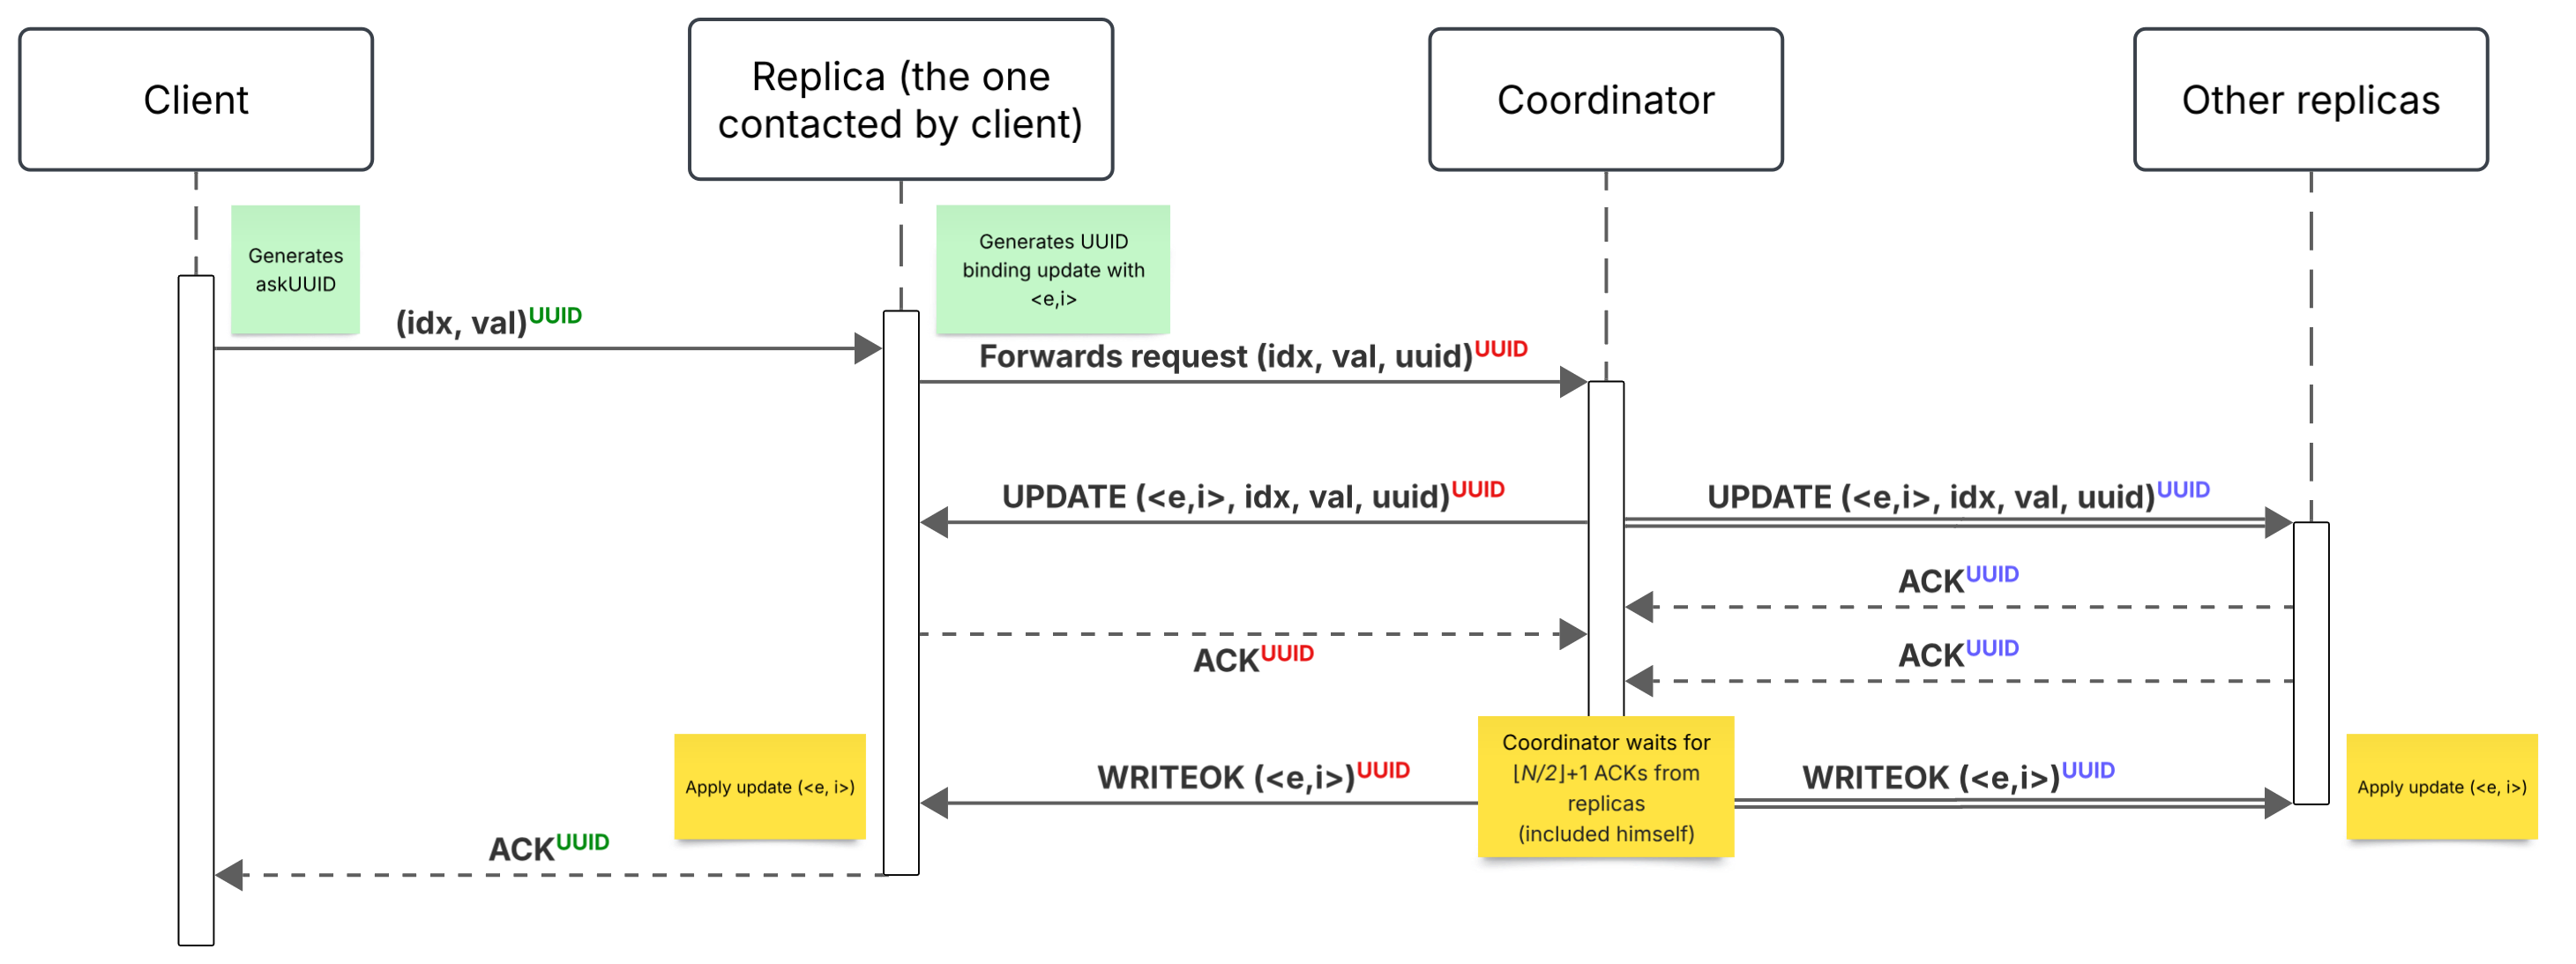
\includegraphics[width=0.5\linewidth]{assets/update_protocol_diagram.png}
                \caption{Update Protocol Diagram}
                \label{fig:protocol_diagram}
            \end{figure}

            To handle timeouts we created a wrapper around \lstinline|tell()| that emulates the behavior of \lstinline|ask()|.

            We initially attempted to follow Akka Ask pattern using the provided \lstinline|ask()| method, which returns a\\
            CompletionStage(future) that completes when a response is received. However, the future is completed on whatever thread delivers the response which is not guaranteed to be the requesting sending actor thread.
            Mutating actor state inside the callback introduce race conditions. \href{https://doc.akka.io/japi/akka-core/2.10/akka/pattern/Patterns.html#ask(akka.actor.ActorRef,java.lang.Object,akka.util.Timeout)}{Akka ask documentation}:
            \textit{"do not call methods or access mutable state [...] from within the callback. This [...] may introduce synchronization bugs and race conditions. [...] there is not yet a way to detect these illegal accesses at compile time."}\\

            The standard solution is to use \lstinline|pipeToSelf|, which delivers the result as a message to the actor mailbox, where it is processed like any other message. 
            But the project requires to use the \lstinline|tell()| method that emulates network latency. And this cannot be done using provided methods.
            
            Therefore we designed our own wrapper called askSystem built on top of the custom \lstinline|tell()| to emulate the ask pattern which makes very easy handling timeouts. AskSystem enables an actor to send messages and register a callback to be executed when a response is received and/or when the specified timeout expires. All messages sent through AskSystem must extend \lstinline|CSAskMessage| which has an UUID as an attribute used to correlate a request with a response and trigger the correct callback.

            When a message is sent a \lstinline|CSAskTimeout| to self is scheduled through a timer. If the response is received in time the timer is canceled and the callback fired, otherwise if the \lstinline|CSAskTimeout| message is received the callback is still fired but with the information that the timer expired.

            Example: Figure \ref{fig:protocol_diagram} where the UUIDs are shown and color coded for each message
        \subsection{Update Protocol}
            The ForwardRequest and the Update message share a UUID which is used to identify the WriteRequest and the corresponding Update which can be confused if two replicas ask to update the same value at the same time.

            Example:
            \begin{itemize}
                \item ReplicaA and replicaB send WriteRequest \lstinline|(index=2, value=7)|
                \item Coordinator sends Update \lstinline|(<0, 1>, index=2, value=7)|
                \item Coordinator sends Update \lstinline|(<0, 2>, index=2, value=7)|
            \end{itemize}
            Which one is the answer to which request? The UUID takes care of matching the Request and the Update
            \subsubsection{Crash Detection}
                During the update protocol the coordinator can detect crashed replicas that do not answer with an Ack.
                
                The coordinator after detecting a crash removes the replica from its list of active replicas and sends a \lstinline|CSCrashNotice| message to the previous replica so that it can update its own list of active replicas and the pointer to the next replica.

                Originally crashed replicas are discovered only during the Election process when passing the message through the ring.
                This extra measure speeds up the Election process avoiding some unnecessary timeouts as crashed replicas can be discovered before the Election.
            \subsection{Updates Logging}
                Update logging is taken care by the class \lstinline|CSUpdateLogger|. Every replica has an attribute \lstinline|updateLogger| which is used to:
                \begin{itemize}
                    \item Log write requests coming from clients
                    \item Log updates coming from the coordinator
                \end{itemize}

                It is important to log also requests as during the coordinator recovery (subsection \ref{subsec:recovery}) we need to process the requests that have not been fulfilled and not only the updates that did not complete.
        \subsection{Coordinator}
            The coordinator acts differently from replicas in almost every operation. We decided to introduce custom behavior than making it behave similarly to replicas as this would have required sending messages to itself.

            As a result all local operations are performed locally skipping the sending of any message.
            \subsubsection{Heartbeat}
                The heartbeat detection is not done through the AskSystem which works only during transactions. We instead opted for a timer based system that in contrast works also during idle periods.

                When a replica becomes a coordinator a recurring self message is scheduled, which upon receiving triggers the broadcast of the heartbeat message to all replicas. Each replica schedules a recurring self message, which triggers a check that the heartbeat has been received during the interval.
                
                A flag is raised when a heartbeat is received and lowered after every check. If the flag is not found raised during a check, an election is initiated.

                The replica start checking for a heartbeat with some delay to allow the coordinator to spin up. In addition the checking interval is a little longer than the beat interval to allow for slowdowns in the communication and processing. Everything combined absorbs propagation delay and avoids false positives.
        \subsection{Election}
            The ring structure needed during the election is maintained through a series of pointers. Each replica has an attribute \lstinline|next| which is a reference to the next Actor in the ring
            \subsubsection{Crash detection}
                When forwarding the election message through the ring if the timeout expires the replica knows that its \lstinline|next| has crashed so it can remove it from its list of active replicas and update its next
            \subsubsection{Non Blocking}
                To make sure that the election process terminates we do two things:
                \begin{itemize}
                    \item If a crash is detected the replica tries to contact the next replica that should be alive and continues indefinitely until the election can continue
                    \item When passing the election message with the chosen coordinator if the previous replica in the ring detects the crash of the winner it removes it from the election message, computes the new winner and continues to circulate the message
                \end{itemize}
        \newpage
        \subsubsection{Recovery} \label{subsec:recovery}
            After sending the synchronization message the coordinator start the recovery of incomplete updates.
            % \begin{enumerate}
            %     \item Computes the oldest update completed across all replicas
            %     \item For each uncompleted update
            %         \begin{itemize}
            %             \item start the update protocol
            %             \item the replica logs it only if it was not already applied
            %         \end{itemize}
            %     \item For each received write request received during the election
            %         \begin{itemize}
            %             \item assign a key in the new epoch to it
            %             \item start the update protocol
            %         \end{itemize}
            % \end{enumerate}

            \begin{algorithm}[H]   
                \textbf{Step 1: compute oldest update completed across all replicas}\\
                \BlankLine
                \textbf{Step 2: send incomplete updates}\\
                \ForEach{update $\in$ incompleteUpdates }{
                    Run the update protocol for \textit{update}
                }
                \BlankLine
                \textbf{Step 3: handle write request received during the election}\\
                \ForEach{writeRequest $\in$ writeRequests}{
                    \textit{update} \(\leftarrow\) create update with a key in the new epoch for \textit{writeRequest}\\
                    Run the update protocol for \textit{update}
                }
            \end{algorithm}
    \section{Implementation}
        \subsection{Custom ask implementation}
            The core of the AskSystem is the \lstinline|ask()| function that emulates the \href{https://doc.akka.io/libraries/akka-core/current/typed/interaction-patterns.html}{Akka ask pattern}.
            The callback is defined with a functional interface (Figure \ref{code:askfinterface}) used to mimic ask original behavior (Figure \ref{code:askoriginal}).
            
            Figure \ref{code:askexample} shows an example of \lstinline|ask()| in use. the return value type is parametric and so casting is automatically performed, \lstinline|res| will be of the type specified.

            \begin{figure}[H]
                \begin{lstlisting}
CompletionStage result = AskPattern.ask(actor, message, timeout);
Figure
result.whenComplete(
    (reply, failure) -> {
        if(...) {...}
        else {...}
    });
                \end{lstlisting}
                \caption{ask in Akka Classic}
                \label{code:askoriginal}
            \end{figure}
            
            \begin{figure}[H]
                \centering
                \begin{lstlisting}
@FunctionalInterface
public interface Callback<T extends CSAskMessage> {
    void handle(T response, boolean timedOut);
}
                \end{lstlisting}
                \caption{ask callback parameter type}
                \label{code:askfinterface}
            \end{figure}

            \begin{figure}[H]
                \begin{lstlisting}
public <T extends CSAskMessage> void ask(
    CSAskMessage msg, ActorRef destination,
    Duration timeout, Callback<T> callback
)
                \end{lstlisting}
                \caption{ask firm}
                \label{code:askfirm}
            \end{figure}

            \begin{figure}[H]
                \begin{lstlisting}
askSystem.<CSUpdate>ask(new CSWriteForward(...),
                replicas.get(this.coordinatorId),
                timeout,
                (res, timedOut) -> {
                    if (!timedOut) {...}
                    else {...}
                }
                \end{lstlisting}
                \caption{ask usage example}
                \label{code:askexample}
            \end{figure}
        \subsubsection{WriteOk Timeout}
            When a replica sends its Ack through ask a timer starts. To avoid the timer from expiring we need to send a WriteOk containing the correct askUUID to the replica.
            The problem is that the coordinator must broadcast the WriteOk message when the quorum is reached.
            
            To comply with AskSystem the coordinator would need to:
            % \begin{itemize}
            %     \item keep track of the askUUIDS associate to the received acks
            %     \item when sending the WriteOk messages
            %         \begin{itemize}
            %             \item send WriteOk with correct askUUIDS to the replicas that partecipated in reaching the quorum
            %             \item send WriteOk with random askUUIDS to other replicas
            %         \end{itemize}
            %     \item answer to every successive ack for that update with a WriteOk with askUUID learned from the ack
            % \end{itemize}

            \begin{algorithm}[H]
                \textbf{Step 1: Collect Acks}\\
                \While{collecting Acks to reach quorum}{
                    Track askUUID associated with received Ack
                }
                \BlankLine
            
                \textbf{Step 2: Send WriteOk messages}\\
                \ForEach{replica $\in$ replicas}{
                    \If{replica participated in reaching the quorum}{
                        Send WriteOk with correct askUUID to \textit{replica}
                    }
                    \Else{
                        Send WriteOk with random askUUID to \textit{replica}
                    }
                }
                \BlankLine
            
                \textbf{Step 3: Answer to successive Acks for the update}\\
                \ForEach{ack $\in$ successiveAcks}{
                    Send WriteOk with askUUID learned from \textit{ack}
                }
            \end{algorithm}
            
            This would work but it would not be very practical and it would require the coordinator to send more messages than the protocol specifies.

            Our solutions instead is for each replica to keep a map of the update key and the askUUID used to send the Ack.
            In \lstinline|HandleUpdate()| the mapping is recorded in \lstinline|Map<CSUpdateKey, UUID> updatesAskUUIDs|.
            Then when the WriteOk message is received it is not feed directly to \lstinline|askSystem.handleResponse()|, previously a new WriteOk message is created with the correct askUUID retrieved from the map.
            
            \begin{lstlisting}
public final void handleWriteOk(CSWriteOk msg) {
    UUID askUUID = this.updatesAskUUIDs.get(msg.getKey());
    this.askSystem.handleResponse(new CSWriteOk(msg.getKey(), askUUID));
}
            \end{lstlisting}
        \subsection{Update Logging}
            We leverage two different HashMaps:
            \begin{itemize}
                \item \lstinline|Map<UUID, CSUpdateData> updates|
                \item \lstinline|Map<CSUpdateKey, UUID> keyToUUIDBindings|
            \end{itemize}

            When a replica receives a WriteRequest from the client the coordinator has not assigned a key yet. The only identifying information is the generated UUID, so the update is first inserted into \lstinline|updates|.

            When replica receives an Update message it binds the key to the UUID through \lstinline|keyToUUIDBindings|.

            Upon receiving the WriteOk which identifies the update only by its key we need to gather the update data chaining the two HashMaps: \lstinline|updates.get(keyToUUIDBindings.get(key))|. The data contains information on the write to apply(index and value) and the reference to the client thaw is waiting for an Ack to the WriteRequest.
    \newpage
    \section{Information about the use of LLM tools}
        \begin{itemize}
            \item Gemini: questions about Java.
            \item ChatGPT: (before starting with the development) questions about the codebase to understand better how to use it.
            \item OpenCode (Big Pickle): reasoning on the codebase and providing pseudo code.
            \item Claude, Mistral: help in writing the report. Used to write drafts and make user that all arguments were covered correctly.
        \end{itemize}
\end{document}
